\documentclass{article}

\usepackage[utf8]{inputenc}
\usepackage[T1]{fontenc}
\usepackage[greek,english]{babel}
\usepackage{alphabeta}
\usepackage{amsmath}
\usepackage{amssymb}
\usepackage{graphicx}
\usepackage{subcaption}
\usepackage{epstopdf}
\usepackage[margin=1in, paperwidth=7.5in,paperheight=10.5in]{geometry}


\newcommand\course{ΤΗΛ513}
\newcommand\courseName{Δορυφορικές Ζεύξεις}
\newcommand\semester{Εαρινό 2020}
\newcommand\assignmentNumber{Lab 1 Δορυφορικών Επικοινωνιών}
\newcommand\studentName{Μαυρογιώργης Δημήτρης}                           
\newcommand\studentNumber{2016030016}

\title{\underline{\textbf{\assignmentNumber}}} 
\author{\textsc{\textbf{Όνομα:}}  \studentName\\
		\textsc{\textbf{ΑΜ:}}  \studentNumber\\
		\course \ - \courseName\\ 
		\textsc{Πολυτεχνείο Κρήτης}
}
\date{\today}
\begin{document}
	\maketitle
\section{Εισαγωγή}
Στόχος της συγκεκριμένης εργασίας είναι η επανάληψη κάποιων βασικών γνώσεων στα Τηλεπικοινωνιακά Συστήματα. Πιο συγκεκριμένα, σε αυτή την εργασία θα μελετήσουμε το bit error rate(BER) της διαμόρφωσης MSK. \\
Όπως είδαμε και στα Τηλεπικοινωνιακά Συστήματα ΙΙ, μπορεί να αποδειχτεί ότι ο μιγαδικός φάκελος της MSK, μπορεί να εκφραστεί ως OQPSK, αν ομαδοποιήσουμε δυάδες ($x_{2n-1},x_{2n}$) διαδοχικών συμβόλων MSK ($x_{n} \in \{\pm1\}$) σε QPSK σύμβολα $x{I,n} + jx_{Q,n} \in \{\pm1 \pm1 \}$. \\
Παράλληλα, μπορεί να δεχτεί ότι το επόμενο σύμβολο QPSK εξαρτάται από τα MSK σύμβολα ($x_{2n-1},x_{2n}$), αλλά και από το προηγούμενο QPSK
σύμβολο σύμφωνα με τις παρακάτω αναδρομικές σχέσεις:
\begin{itemize}
	\item $ x_{I,n} = -x_{Q,n-1} \cdot x_{2n-1}$
	\item $ x_{Q,n} = -x_{I,n} \cdot x_{2n}$	
	\item $ x_{Q,-1} =-1 $ και $x_{-1}=1$
\end{itemize}
Εν ολίγοις, παρατηρούμε ότι η MSK, μπορεί να θεωρηθεί μια OQPSK με μνήμη, εφόσον για τον υπολογισμό των  συμβόλων QPSK χρησιμοποιούνται οι παραπάνω αναδρομικοί τύποι.  

\section{Eρώτημα Α}
Oρίζουμε τη σηματοθορυβική σχέση ως εξής:
$$SNR = \frac{A^2T}{β}$$ 
όπου β ειναι η φασματική πυκνότητα ισχύος $S_{wwI} = S_{wwQ} = β$\\
Για SNR = 5 dB και $Ν=10^5$ bits, προσομοιώνουμε την παρακάτω εξίσωση: 
$$y_{n} = ATz_{n} + \sqrt{βT}n_{n}$$
όπου $z_{n} = x_{I,n} +jx_{Q,n}$ τα συμβολα QPSK και $n_{n} = n_{I,n} +jn_{Q,n}$ μια κυκλικώς συμμετρική Γκαουσιανή $n_{n} \sim N(0,2)$\\
Aπό την προσομοίωση στο Matlab εκτημήθηκε ότι το bit error rate της MSK είναι περίπου ίσο με 0.07129.\\
\section{Eρώτημα Β}
Για τιμές SNR=6 εως 12 dB προκύπει το παρακάτω αποτέλεσμα:\\
\begin{figure}[h]
	\centering
	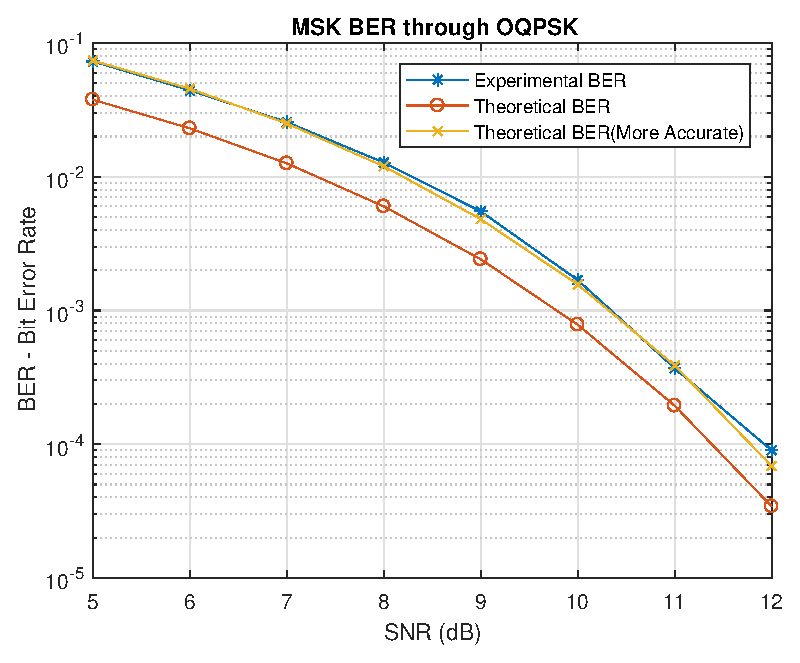
\includegraphics[width=0.8\linewidth]{./results/epsFig}
	\caption{BER for different SNR(dB)}
\end{figure}
\section{Eρώτημα Γ}
Από τo παραπάνω διάγραμμα (figure 1) παρατηρούμε ότι αν θεωρήσουμε $P_{b} = Q(\sqrt{SNR})$ δε συμπίπτουν μεταξύ τους η θεωρητική με την πειραματική καμπύλη, αλλα έχουν μια μικρή απόκλιση. \\
Πιο συγκεκριμένα, το BER της προσομοίωσης είναι ελάχιστα χειρότερο από το θεωρητικό. Eπομένως, μπορούμε να θεωρήσουμε ότι η σχέση $P_{b} = Q(\sqrt{SNR})$ αποτελεί μια προσέγγιση του BER της MSK.\\
Ωστόσο, το BER της MSK δεν ισούται ακριβώς με $Q(\sqrt{SNR})$, καθώς η διαμόρφωση QPSK χρησιμοποιεί μνήμη, καθώς για τον υπολογισμό των επόμενων συυμβόλων χρησιμοποιείται το προηγόυμενο.
\section{Eρώτημα Δ}
Γενικότερα, για το symbol error rate της QPSK(M=4) ισχύει ότι:\\
$$P_{M}= 1 - (1 - P_{\sqrt{M}} )^2 = 
1 - (1 - Q(\sqrt{SNR}) )^2 = 
2 \cdot  Q(\sqrt{SNR}) - [Q(\sqrt{SNR})]^2$$ \\

\noindent
Ωστόσο, σωστό σύμβολο μπορούμε να λάβουμε αν ληφθούν ταυτόχρονα λάθος τα $x_{I,n}$, $x_{Q,n}$. Για παράδειγμα και χωρίς να υπάρχει βλάβη της γενικότητας, αν έχουμε το σύμβολο 1+j1 μπορούμε να λάβουμε τα σωστά 2 MSK bits, ακόμα και αν λάβουμε το σύμβολο -1-j1.\\
Συνεπώς, για τη συγκεκριμένη OQPSK με μνήμη το συνολικό SER είναι:
$$P_{E}= 2 \cdot P_{M}$$.
Aν διαιρέσουμε και με το $\log_2 M = \log_2 4 = 2$, έχουμε ότι ακριβές το BER της MSK έιναι:
$$P_{b}= P_{M} = 2 \cdot  Q(\sqrt{SNR}) - [Q(\sqrt{SNR})]^2$$.
\section{Eρώτημα Ε}
Το λαμβανόμενο σήμα αποδιαμορφώνεται σαν την QAM και δίνει τα σήματα βασικής ζώνης $s_{I}(t)$ και $s_{Q}(t)$ στις εξόδους των δύο βαθυπερατών φίλτρων. \\
Έπειτα, τα $s_{I}(t)$ και $s_{Q}(t)$ περνούν μέσα από ένα προσαρμοσμένο φίλτρο, δηλαδή πολλαπλασιάζονται με $cos\left(\frac{πt}{2T_{b}}\right)$ και $sin\left(\frac{πt}{2T_{b}}\right)$ αντίστοιχα, και ολοκληρώνονται στις αντίστοιχες περιόδους, με αποτέλεσμα να δίνουν στην έξοδο τα $a_{Ι}$  και $a_{Q}$, τα οποία είναι τα άρτια και περιττά σύμβολα MSK αντίστοιχα.


\begin{figure}[h]
	\centering
	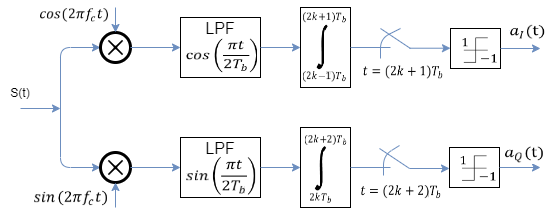
\includegraphics[width=0.8\linewidth]{./results/MSK_detector.png}
	\caption{MSK detection block diagram}
\end{figure}
\section{Eρώτημα ΣΤ}
Πριν την αποστολή των bits της MSK γίνεται χρήση ενός διαφορικού προκωδικοποιητή  στην είσοδο του πομπού και αντίστοιχου αποκωδικοποιητή στην έξοδο του δέκτη.\\ Ειδικότερα, υπολογίζουμε την προκωδικωποιημένη ακολουθία bits στο δέκτη ως εξής:
$$b[n] = a[n] \oplus a[n-1]$$
όπου a[n] είναι η ακολουθία bits MSK πριν την κωδικοποίηση.\\
Επίσης, η αποκωδικοποιημένη ακολουθία bits MSK στο δέκτη υπολογίζεται ως εξής:
$$a[n] = b[n] \oplus a[n-1]$$
όπου b[n] είναι τα ληφθέντα bit MSK πριν την αποκωδικοποίηση.\\
Με τη χρήση του παραπάνω precoding  κάθε εσφαλμένο bit της b[n], γίνεται ένα μονό εσφαλμένο bit στην έξοδο του αποκωδικοποιητή, με την προυπόθεση ότι τυχόν σφάλματα των bI και bQ να μην είναι συνεχόμενα. 
\end{document}
